%% LyX 2.2.2 created this file.  For more info, see http://www.lyx.org/.
%% Do not edit unless you really know what you are doing.
\documentclass[11pt,english]{beamer}
\usepackage{enumerate}
\usepackage{float}
\usepackage{mathptmx}
\usepackage[T1]{fontenc}
\usepackage[utf8]{inputenc}
\setlength{\parskip}{\smallskipamount}
\setlength{\parindent}{0pt}
\usepackage{url}
\usepackage[authoryear]{natbib}
\usefonttheme[onlymath]{serif} % para las fuentes de las ecuaciones
\makeatletter
\usepackage{amsmath,amssymb,amsthm}
\usepackage{graphicx}
\usepackage{xcolor} % para colorear textos con \textcolor o \color
\usepackage{hyperref}
\usepackage{times}
\usepackage{array}
\usepackage{multicol}
\usepackage{longtable}
\usepackage{float} % para usar comando [H] en tablas y gr\'aficas
\usepackage{xcolor}% para modificar el color de la presentacion y del texto
\usepackage{colortbl} % para tablas de Kable
\usepackage{booktabs} % Para toprule: To thicken table lines 
\usepackage[nogin]{Sweave} % elimina el tamaño por default de las figuras de sweave
\usepackage{natbib}
\bibliographystyle{agsm}
% \usepackage[inline]{enumitem} % para enumerar dentro de un paragrafo
\usepackage{rotating} % para rotar nombres de columnas

\usepackage{graphicx}
\usepackage{subcaption}

\usepackage{listings} % esta y la siguiente para resolver el problema del FancyVerb 
\lstset{basicstyle=\ttfamily} % esta tambien para lo del FancyVerb 



%%%%%%%%%%%%%%%%%%%%%%%%%%%%%% LyX specific LaTeX commands.
\providecommand{\LyX}{L\kern-.1667em\lower.25em\hbox{Y}\kern-.125emX\@}

%%%%%%%%%%%%%%%%%%%%%%%%%%%%%% Textclass specific LaTeX commands.
 % this default might be overridden by plain title style
 \newcommand\makebeamertitle{\frame{\maketitle}}%
 % (ERT) argument for the TOC
 \AtBeginDocument{%
   \let\origtableofcontents=\tableofcontents
   \def\tableofcontents{\@ifnextchar[{\origtableofcontents}{\gobbletableofcontents}}
   \def\gobbletableofcontents#1{\origtableofcontents}
 }
\newcommand{\code}[1]{\texttt{#1}}

%%%%%%%%%%%%%%%%%%%%%%%%%%%%%% User specified LaTeX commands.
\usetheme{CambridgeUS}
% or ...
% Define new colors for background and foreground
\setbeamercolor{background canvas}{bg=white} % Change to your desired color
\setbeamercolor{title}{fg=white}              % Set the title text color, if needed
\setbeamercolor{frametitle}{bg=green, fg=white} % Change frame title color
\setbeamercovered{transparent}
% or whatever (possibly just delete it)

\usepackage[T1]{fontenc}
\usepackage{lmodern}
\makeatother

\usepackage{babel}
\usepackage{listings}
\renewcommand{\lstlistingname}{\inputencoding{latin9}Listing}

\begin{document}
\Sconcordance{concordance:5_ACP_19_04_2026_diapositivas.tex:5_ACP_19_04_2026_diapositivas.Rnw:1 %
51 1 1 4 351 1 1 8 3 1 1 7 14 0 1 2 9 1 2 2 168 1 1 11 1 1 1 7 28 0 1 2 %
2 1 1 6 4 1 1 6 1 2 4 1 1 8 14 0 1 2 5 1 1 3 1 2 4 1 1 8 12 0 1 2 3 1 1 %
6 12 0 1 2 2 1 1 5 12 0 1 2 14 1 1 9 27 0 1 2 2 1 1 5 27 0 1 2 2 1 1 5 %
27 0 1 2 5 1 1 3 1 2 7 1 2 2 16 1 1 4 5 1 2 2 19 1 1 10 1 1 1 16 19 0 1 %
2 5 1 2 2 3 1 1 12 3 1 1 6 26 0 1 2 1 1 1 4 4 1 2 2 64 1 1 8 24 0 1 2 7 %
1 1 6 45 1}



\title{Análisis de Componentes Principales (ACP)}

\subtitle{Introducción}

\author{Jimmy A Corzo S\inst{1} \inst{2}}

\institute[Profesor Titular]{\inst{1}Profesor Titular\\
Departamento de Estadística\and \inst{2}Facultad de ciencias\\
Universidad Nacional de colombia}

\date[2023]{Métodos multivariados aplicados \LyX{} cap 3}

\makebeamertitle

%\pgfdeclareimage[height=0.5cm]{institution-logo}{institution-logo-filename}

%\logo{\pgfuseimage{institution-logo}}

\AtBeginSubsection[]{

  \frame<beamer>{ 

    \frametitle{Outline}   

    \tableofcontents[currentsection,currentsubsection] 

  }

}

%\beamerdefaultoverlayspecification{<+->}
\begin{frame}
\tableofcontents{}
\end{frame}

\section{Descripción del método}
\begin{frame}{Dos enfoques de las componentes principales}
La manera más común entre estadísticos de ver el Análisis de Componentes Principales es como un método de buscar ponderaciones apropiadas para construir combinaciones lineales (sumas ponderadas) de las variables $X_1,\ldots,X_p$ que acumulan la mayor cantidad posible de varianza de la tabla de datos, combinaciones que son ortogonales por construcción, lo que carantiza que no están correlacionadas.\vskip5mm

Un segundo enfoque es el desde el aprendizaje estadístico, en la cual la búsqueda de las componentes es un problema de optimización que consiste en encontrar la mejor aproximación de la matriz de datos, minimizando las sumas de cuadrados de las diferencias entre las observaciones y sus aproximaciones.

\end{frame}

\section{Descripción del método}
\begin{frame}{Dos enfoques de las componentes principales}

Los dos enfoques producen la misma solución, debido a que la aproximación buscada por minimización de las sumas cuadrados, corresponde a la solución dada por el Teorema de la Descomposición en Valores Singulares para la reconstrucción de la matriz de datos a partir de los valores y vectores propios de $X^\prime X$ y de $XX^\prime$, la cual produce las componentes en las direcciones de máxima varianza de $X$.
\end{frame}
% 
\begin{frame}{Descripción del método}
\small
Éstas combinaciones lineales se denominan \textbf{componentes principales, factores o dimensiones}. Luego se utilizan unas cuantas de ellas para comprender mejor los datos, analizar y visualizar tablas de datos, para reduccion de dimensiones, para visualización o imputación de datos faltantes entre otras de sus aplicaciones. 
\vskip1mm
En el contexto de regresión las componentes suelen utilizarse como predictores cuando hay problemas de multicolinealidad.
\vskip1mm
El ACP es la base de los llamados Métodos Factoriales entre los que se cuentan también el Análisis de Correspondencias Simples, el Análisis de Correspondencias Múltiples (ACM) y varias generalizaciones de éstos para tablas múltiples o tablas de tres índices en las cuales se pueden mezclar tablas de variables cuantitativas y tablas de variables cualitativas.

\end{frame}
% 
\begin{frame}{Descripción del método}
El ACP se cuenta entre los métodos no supervisados puesto que incluye solamente datos de las variables o caracteristicas $X_1,\ldots,X_p$ observadas en los objetos, sin una respuesta asociada sobre la cual se pueda supervisar la calidad de los resultados que producen, y por tanto tampoco se pueden hacer predicciones de ningún tipo.
\vskip1mm
Por esta razón, se muestra también un enfoque dentro del moderno aprendizaje estadistico no supervisado que utiliza las componentes para aproximar la matriz de datos y permite calcular los errores en la aproximación como errores residuales de ésta.


\end{frame}
% 
\begin{frame}{Utilidad del ACP}
Suele ser útil entre muchas aplicaciones, para 
\begin{itemize}
	\item reduccion de dimensiones
	\item imputación de datos faltantes
	\item en el contexto de regresión las componentes se pueden utilizar como predictores.
	\item para visualización de tablas de datos
	\item exploración y análisis de tablas de datos
\end{itemize}
\end{frame}

\begin{frame}{Utilidad del ACP}
El ACP es la base de los llamados Métodos Factoriales entre los que se cuentan también \vskip1mm
* Análisis de Correspondencias Simples (ACS)\vskip1mm
* Análisis de Correspondencias Múltiples (ACM)\vskip1mm
* Generalizaciones de ACP, ACS y ACM para tablas múltiples o de tres índices en las cuales se pueden mezclar tablas de variables cuantitativas y de variables cualitativas\vskip1mm
* Métodos de agrupamiento (Métodos Jerárquicos)
% , los cuales \textbf{utilizan las componentes llamadas factores en un contexto más general} para analizar y visualizar varias tablas de datos de variables cuantitativas o cualitativas.
\end{frame}


\begin{frame}{Definición y propiedades de las componentes principales como direcciones de máxima varianza de la matriz de datos}
\textbf{Matriz de datos centrados, estandarizados y normados}
\begin{align}\label{Y_c_est}
	Y = \frac{1}{\sqrt{n}}\widetilde{Y} = \frac{1}{\sqrt{n}} \widetilde{X} D^{-1/2}
\end{align}
la cual tambien está centrada puesto que 
$$
med(Y) = \frac{1}{\sqrt{n}}med(\widetilde{Y}) = 0
$$
y por estar autoponderada por $\frac{1}{\sqrt{n}}$ el producto consigo misma es su matriz de covarianzas y también la matriz de correlación:
\begin{equation}
	S_{Y} = Y^\prime Y = \frac1n \widetilde{Y}^\prime \widetilde{Y} = R.
\end{equation}
\end{frame}
% 
\begin{frame}{Aplicación del TDVS}
\small
El TDVS aplicado a la matriz de datos centrados estandarizados y normados $Y$ produce la siguiente expresión para reconstruirla:
\begin{equation}\label{eq:svdY_113}
Y = U L V',
\end{equation}
donde
\begin{align*}
&	U \, \text{y} \, V \text{son matrices con columnas ortonormales, lo cual implica }\, U'U = V'V = I\\
& L_{p\times p}=\mathrm{diag}\!\left(\sqrt{\lambda_\alpha}\right),\, \lambda_\alpha \ge 0,\, \lambda_1 \ge \cdots\ge\lambda_p,
\,\, \lambda_\alpha \ \text{es el $\alpha$-ésimo valor propio de } Y'Y,\ \alpha=1,\ldots,p,
\end{align*}
\begin{align*}
	V_{p\times p} &=\left(v_1,\ldots,v_p\right), \quad
	v_\alpha=\left(v_{1\alpha},\ldots,v_{p\alpha}\right)' \ \text{es el $\alpha$-ésimo vector propio de } Y'Y=R,\\
	& \text{y define las 
		\emph{direcciones ortogonales de máxima varianza} }\\
	&	\text{en el \emph{espacio de las variables}
		(\emph{cargas factoriales} o \emph{loadings} de las variables);}
\end{align*}
\begin{align*}
	U_{n\times p}&=\left(u_1,\ldots,u_p\right), \quad
	u_\alpha=\left(u_{1\alpha},\ldots,u_{n\alpha}\right)' \ \text{es el $\alpha$-ésimo vector propio de } YY',\\
	& \text{y define las 
		\emph{direcciones ortogonales de máxima varianza}}\\
	&	\text{en el \emph{espacio de los objetos}.
		(\emph{cargas factoriales} o \emph{loadings} de las objetos);}
\end{align*}
\end{frame}
% 
\begin{frame}{xxxx}
Se define la matriz de componentes principales como el producto
\begin{equation}\label{eq:Z_114}
Z = YV 
\end{equation}
donde las columnas de $Z$ son las \emph{componentes principales} (o \emph{scores}) de los objetos,
y $V$ contiene las direcciones de máxima varianza. Este producto se denomina  matriz de componentes principales para los objetos, pues representa las proyecciones de los valores de los objetos en las variables sobre los vectores propios de $Y'Y$.
\end{frame}
% 
\begin{frame}{xxxx}
Nótese que las componentes principales estan centradas
\begin{equation}
	med(Z) = \frac1n Z' \mathbf{1_n} =  V' \frac1n Y' \mathbf{1_n} = V' \cdot 0 = 0,
\end{equation}
puesto que $\frac1n Y' \mathbf{1_n} = med(Y) = 0$.

También se puede demostrar que la matriz de covarianzas de $Z$ es (ver por ejemplo \cite{husson2017exploratory}):
\begin{equation}
	Z'Z = \Lambda, \quad \text{donde}\quad 	\Lambda=\operatorname{diag}(\lambda_1,\ldots,\lambda_p),
\end{equation}
lo cual indica que las componentes son incorrelacionadas y que sus varianzas son los valores propios de $Y'Y$.
\end{frame}
% 
\begin{frame}{Análisis para los objetos.}

Particionando la matriz $V$ por columnas, $V=(v_1,\ldots,v_p),\quad \text{donde} \, v_\alpha = (v_{1\alpha}, \ldots, v_{p\alpha})$ se obtiene:
% \in\mathbb{R}^{p}
\begin{equation*}
	Z=YV = \bigl(Yv_1,\ldots,Yv_p\bigr),
\end{equation*}
de manera que la $\alpha$-ésima columna de $Z$ es el vector:
    \begin{equation}\label{alphaesima_cp}
	z_\alpha = Y v_\alpha \quad \text{para } \alpha=1, \dots, p
    \end{equation}
que se define como la $\alpha$ - ésima componente principal, en la cual se ve claramente que  \textcolor{blue}{$z_\alpha$ es la proyección de las observaciones de los objetos (filas de $Y$) en la dirección de $v_\alpha$}. Por tanto, $Z_1$ va en la dirección de $v_1$ que es el vector ropio asociado a $\lambda_1$ el mayor valor propio de $Y'Y$; $Z_2$ va en la dirección de $v_2$ el vector propio asociado a $\lambda_2$ el segundo mayor valor propio de $Y'Y$, y así sucesivamente. 
\end{frame}
% 
\begin{frame}{Análisis para los objetos.}
En particular, definiendo la $i$-ésima fila de $Y$ por $y_{i.} = (y_{i1},\ldots,y_{ip})$,  las cooordenadas para el objeto $i$ sobre la $\alpha$ - ésima componente principal son:
    $$z_{i\alpha} = y'_{i.} v_\alpha = \sum_{j=1}^p y_{ij}\,v_{j\alpha}, \qquad i=1,\ldots,n.$$

Finalmente, su varianza está dada por
\[
\mathrm{var}(Z_\alpha)=\frac{1}{n}\sum_{i=1}^n z_{i\alpha}^2
=\frac{1}{n}v_\alpha'Y'Yv_\alpha
=\frac{1}{n}\lambda_\alpha,
\]
lo cual es consistente con la normalización adoptada en la construcción de $Y$.
\end{frame}
% 
\begin{frame}{Análisis para las variables}

Por otra parte, obsérvese que, a partir del TDVS de $Y$ dado en \eqref{eq:svdY_113},
\[
Y = U L V',
\]
se tiene
\[
Y' = V L U'.
\]
Entonces, al multiplicar $Y'$ a derecha por $U$ se obtiene
\begin{equation}\label{eq:W_117}
W = Y'U = V L \qquad \text{para las variables}.
\end{equation}

Por tanto, la $\alpha$-ésima componente principal asociada al $\alpha$-ésimo vector propio
$u_\alpha$ de $YY'$ viene dada por
\begin{equation}\label{eq:Wa_118}
W_\alpha = Y'u_\alpha, 
\qquad \alpha = 1,\ldots,p,
\quad \text{para las variables}.
\end{equation}


\end{frame}
% 
\begin{frame}{Análisis para las variables}
Las coordenadas de las variables sobre la $\alpha$-ésima componente principal son, por tanto,
\begin{equation}\label{eq:waj_119}
w_{\alpha j}
=
\sum_{i=1}^n u_{i\alpha}\, y_{ij},
\qquad j = 1,\ldots,p.
\end{equation}

En este caso, los elementos del vector
\[
u_\alpha = (u_{1\alpha},\ldots,u_{n\alpha})'
\]
definen las direcciones ortogonales de máxima varianza en el espacio de los objetos.
Las cantidades $w_{\alpha j}$ representan las coordenadas de la variable $j$ sobre la
$\alpha$-ésima componente principal, y describen cómo cada variable se asocia con las
direcciones principales determinadas por la variabilidad conjunta de los objetos.
\end{frame}
% 
\begin{frame}{Proporción de varianza explicada por las primeras $q$ compontes}
Se obtiene utilizando el hecho de que la varianza total es la suma de los $p$ valores propios de $R$ y por tanto la proporción explicada por los primeros $q$ es:
\begin{equation}\label{PctVarValPropios1}
\tau_r=\frac{\sum_{\alpha=1}^{q}\lambda_\alpha}{\sum_{\alpha=1}^{p}\lambda_\alpha}
\end{equation}
En este enfoque, el ACP consiste básicamente en buscar una representación óptima de la matriz de datos centrados, estandarizados y normados $Y_{n \times p}$ mediante $q$\ ($<p$) combinaciones lineales (o promedios ponderados) llamadas componentes principales\footnote{El método fue presentado inicialmente por \cite{pearson1901principal} y desarrollada por \cite{hotelling1933analysis}}. 
\end{frame}
% 
\begin{frame}{Proporción de varianza explicada por las primeras $q$ compontes}
Lo óptimo se refiere por una parte a que por estar calculadas en las direcciones de máxima varianza de $Y$  las $q$ componentes utilizadas para la representación contienen la mayor cantidad posible de la varianza de la matriz de datos $Y_{n\times p} $,\ y en segundo lugar a que dichas componentes son perpendiculares (ortogonales) entre sí. En este sentido, las componentes principales son una forma de reducir las dimensiones de análisis de $p$ variables a $q$ componentes que  facilitan los análisis y la interpretación, y permiten visualizar objetos y variables.\\
\end{frame}
% 
\begin{frame}{Ecuaciones de transición entre el análisis para objetos y el análisis para variables}
\small
Para construir las  ecuaciones de transición se requiere el siguiente resultado.
Sea \(u_\alpha\) es un vector propio de \(Y'Y\) asociado a un valor
propio no nulo \(\lambda_\alpha\), entonces:
\begin{equation}
	Y'Y\,u_\alpha = \lambda_\alpha u_\alpha, \quad \text{con} \quad \lambda_\alpha \neq 0
\end{equation}
Al multiplicar a izquierda por \(Y\) y reagrupar se obtiene
\begin{equation}
	YY'(Yu_\alpha) = \lambda_\alpha (Yu_\alpha).
\end{equation}
Como \(\lambda_\alpha \neq 0\), se sigue que \(Yu_\alpha \neq 0\), y por tanto
\(\lambda_\alpha\) es también un valor propio de \(YY'\).

El razonamiento inverso se obtiene de manera análoga, lo que permite concluir que
las matrices \(Y'Y\) y \(YY'\) comparten los mismos valores propios no nulos. En
consecuencia, denotando por \(\lambda_\alpha\) y \(\mu_\alpha\) los valores
propios no nulos de \(Y'Y\) y \(YY'\), respectivamente, se cumple que
\begin{equation}
	\lambda_\alpha = \mu_\alpha,
	\qquad \alpha = 1,\ldots,r,
\end{equation}
donde \(r=\mathrm{rango}(Y)\) (número de columnas linealmente independientes de $Y$).
\end{frame}
% 
\begin{frame}{Ecuaciones de transición entre el análisis para objetos y el análisis para variables}
\small
La transición entre los espacios de objetos y variables se obtiene utilizando el hecho de que
% Premultiplicando en (\ref{TrCoPr2_z}) por $Y$ se obtiene:
\begin{equation}
	(Y^\prime Y) u_\alpha = R u_\alpha = \lambda_\alpha u_\alpha
\end{equation}
Entonces multiplicando a izquierda por $Y$ y reagrupando términos se obtiene:
\begin{equation}\label{transicio_u}
	YY^\prime (Y u_\alpha) = \lambda_\alpha (Y u_\alpha)
\end{equation}


lo cual indica que $Yu_\alpha$ es un vector propio de $YY^\prime$ respecto al valor propio $\lambda_\alpha$. Por otra parte, como la norma de $Yu_\alpha$ es $u_\alpha^\prime Y^\prime Yu_\alpha = \lambda_\alpha $ entonces el vector:
\begin{equation}\label{v_normado}
	v_\alpha = \frac{1}{\sqrt{\lambda_\alpha}}Yu_\alpha 
\end{equation}
es un vector propio normado de $YY^\prime$ respecto al valor propio $\lambda_\alpha$.
\end{frame}
% 
\begin{frame}{Ecuaciones de transición entre el análisis para objetos y el análisis para variables}
\small
Análogamente, se utiliza el hecho de que 
\begin{align}
	YY'v_\alpha = \mu_\alpha v_\alpha, \text{donde }\, \mu_\alpha \, \text{es un valor propio de } YY'
\end{align}
de manera que al premultiplicar por $Y'$ y reagrupando se obtiene:
\begin{equation}
	Y'Y(Y^\prime v_\alpha) = \mu_\alpha (Y^\prime v_\alpha)
\end{equation}
y por tanto $Y^\prime v_\alpha$ es un vector propio de $Y^\prime Y$ respecto al valor propio $\mu_\alpha$. También en este caso la norma de $u_\alpha = Y^\prime v_\alpha$ es $\mu_\alpha = \lambda_\alpha $. Entonces, 
\begin{equation}\label{transicio_v}
	u_\alpha =  \frac{1}{\sqrt{\lambda_\alpha}}Y^\prime v_\alpha
\end{equation}
es un vector propio normado de $Y^\prime Y$ respecto al valor propio $\lambda_\alpha$. Entonces
\begin{equation}
	z_\alpha = Yu_\alpha = \frac{1}{\sqrt{\lambda_\alpha}} Y Y^\prime v_\alpha = \sqrt{\lambda_\alpha}v_\alpha
\end{equation}
\textcolor{blue}{La conclusión es que es suficiente con calcular valores y vectores propios de $Y^\prime Y$, pues a partir de éstos se pueden obtener los de $YY^\prime$ y viceversa.}
\end{frame}
% 
\begin{frame}{Ayudas para la interpretación}
\LARGE
APLICACIONES
\end{frame}
% 
\section{Ejemplos}
\begin{frame}{Ejemplo indicadores de invest. y cobertura en educ. superior ciudades }
Para el archivo de indicadores de ciudades un ACP de los siguientes indicadores

"N.Gr.Inv..Colciencias", 

"No.CeNTROS.Inv", 

"No.Prf..Doctorado", 

"Poblacion" y  

"Cobertura.ed.sup". 
\end{frame}



% ________________________________________________________
\begin{frame}{Ejemplo indicadores de invest. y cobertura en educ. superior ciudades }
\small
\begin{table}[!h]
\centering
\caption{\label{tab:Ciucompleto}Indicadores de calidad de las componentes}
\centering
\begin{tabular}[t]{lrrr}
\toprule
  & eigenvalue & percent of variance & cum percent of variance\\
\midrule
\cellcolor{gray!10}{comp 1} & \cellcolor{gray!10}{2.96} & \cellcolor{gray!10}{59.29} & \cellcolor{gray!10}{59.29}\\
comp 2 & 1.40 & 27.91 & 87.20\\
\cellcolor{gray!10}{comp 3} & \cellcolor{gray!10}{0.34} & \cellcolor{gray!10}{6.73} & \cellcolor{gray!10}{93.93}\\
comp 4 & 0.17 & 3.46 & 97.39\\
\cellcolor{gray!10}{comp 5} & \cellcolor{gray!10}{0.13} & \cellcolor{gray!10}{2.61} & \cellcolor{gray!10}{100.00}\\
\bottomrule
\end{tabular}
\end{table}\vskip-1mm

Las dos primeras dos comp aportan $\lambda = 87.2\% $ de la varianza indicando una buena aproximación (ver $3^a$ columna de la tabla \ref{tab:Ciucompleto}).
\end{frame}

% ________________________________________________________
\begin{frame}{Ejemplo indicadores de invest. y cobertura en educ. superior ciudades }
\setkeys{Gin}{width=0.8\textwidth} % redefinir el tamaño graficos
\begin{figure}[H]
	\centering
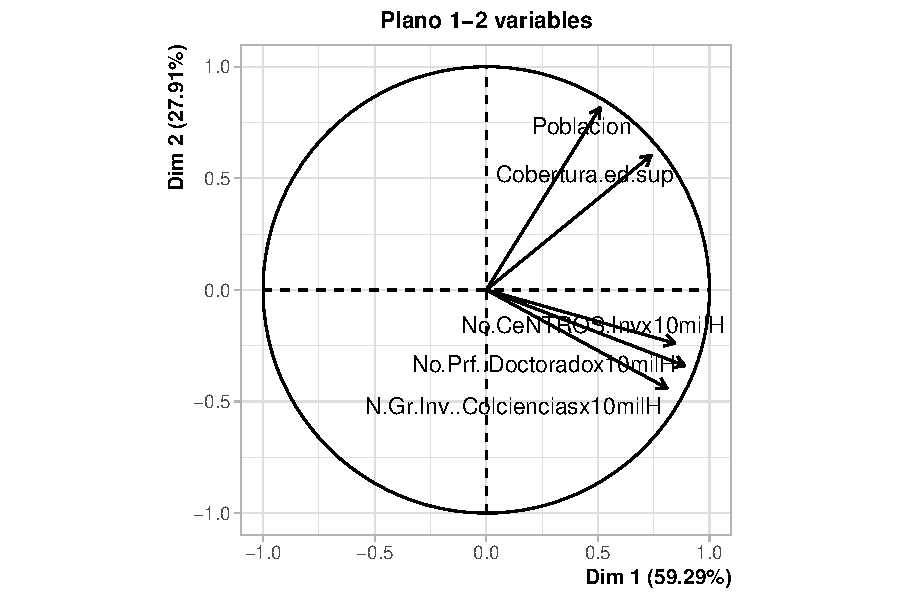
\includegraphics{5_ACP_19_04_2026_diapositivas-004}
	\caption{Indicadores de educación superior sobre las dos primeras componentes}\label{fig:edSuperiorl}
\end{figure}
Las dos primeras dos componentes aportan $\lambda = 87.2\% $ de la varianza indicando una buena aproximación.
\end{frame}
% __________________________________________________________

% \begin{frame}{Ejemplo indicadores de invest. y cobertura en educ. superior ciudades }
% \setkeys{Gin}{width=0.8\textwidth} % redefinir el tamaño graficos
% \begin{figure}[H]
% 	\centering
% <<fig=T, echo=F, height=4, width=6>>=
% require(FactoMineR)
% plot.PCA(pca_ciudCompl, choix = "ind", title = "Plano 1-2 variables")
% @
% 	\caption{Ciudades sobre el plano de indicadores de educación superior}\label{fig:edSuperiorl}
% \end{figure}
% Los dos primeros factores aportan $\lambda = 87.2\% $ de la varianza indicando una buena aproximación.
% \end{frame}
\begin{frame}{Guías para la interpretación del ACP}
\LARGE
Guías para la interpretación del ACP
\end{frame}


\section{Guías para la interpretación del ACP}
\begin{frame}{Guías para la interpretación del ACP: Calidad de la representación}
\begin{itemize}
	\item \textbf{Calidad de la representación.} Porcentaje de varianza acumulada por las $Q$ componentes escogidas para la representación en menos dimensiones. Denotando por $\lambda_\alpha = v(z_\alpha)$ la varianza de la $\alpha$ - ésima componente, el procentaje de varianza acumulado por las primeros $Q$ componentes se calcula por:
  	\begin{equation}
\tau_Q=\frac{\sum_{\alpha=1}^{Q}\lambda_\alpha}{\sum_{i=1}^{p}\lambda_\alpha}
    \end{equation}
\end{itemize}
\end{frame}
% 
\begin{frame}{Guías: Calidad de la representación}
Entonces la calidad depende de una buena selección de $Q$ el número de factores, para lo cual existen variados criterios en la lieratura entre los que se pueden mencionar dos frecuentemente utilizados:
      \begin {itemize}
    	\item Utilizar tantos como sean necesarios para alcanzar un porcentaje de varianza prefijado;
    	\item Escoger todos aquellos que sean mayores que uno. (Otros criterios se pueden ver en \cite{eastment1982cross}, \cite{josse2012selecting});
      \end {itemize}
\end{frame}

\begin{frame}{Guías: Correlaciones variable-factor.}
\textbf{Correlaciones variable-factor.} Son indicadores del grado en que una variable explica un factor. 

Para el $\alpha$ - ésimo factor esta correlación es  $$\sqrt{\lambda_\alpha} u_{j\alpha}$$. 

Entre más alta la correlación variable-factor, mejor explicado queda el factor por la variable. \label{corvariablefactor}
\end{frame}

\begin{frame}{Guías: Tipificación de los factores}
\textbf{Tipificación de los factores (componentes) por las variables.}
	Para la tipificación de los factores se utilizan los siguientes indicadores que relacionan las posiciones de las variables con respecto a los ejes que forman planos factoriales:
  \begin{itemize}
        \item \textit{Coordenadas (scores):} Posiciones de las variables en los planos factoriales defindas en \ref{ec:facto1}. Puesto que los factores se construyen sobre la matriz de correlación, coinciden con las correlaciones variable factor. La única forma que no coincidan es que el ACP sea realizado sobre la matriz de covarianzas.
  \end{itemize}
\end{frame}

\begin{frame}{..}
\begin{itemize}
	\item \textit{Contribuciones a la varianza de los factores:} 
	
        	Como $\lambda_\alpha = v(z_\alpha) = \sum_{j=1}^p z_{\alpha j}^2$ entonces         	\[
        	\frac{z_{\alpha j}^2}{\lambda_\alpha} 
        	\]
\end{itemize}
Es decir, la contribución de la variable $j$ a la varianza del factor  $\alpha$ es la proporción de varianza que aporta la variable $j$ a la suma.
\end{frame}

\begin{frame}{..}
\begin{itemize}
	\item \textit{Cosenos cuadrados (cos2):} Capacidad de los factores para predecir las variables. Sea $\theta_{j,\alpha}$ el ángulo entre la variable $j$ y la componente $z_\alpha$. Entonces el coseno al cuadrado $\theta_{j,\alpha}$ es la correlación variable-factor elevada al cuadrado representa la cantidad de varianza de la variable que está explicada por el factor:
\begin{equation} \label{coseno}
cos^2(\theta_{j,\alpha}) = \lambda_\alpha u^2_{j\alpha}
\end{equation}
Puede ocurrir en algunas aplicaciones que una variable tenga alta contribución y alta correlación con un factor, pero sus cosenos cuadrados no son suficientemente altos para que dicho factor sea un buen predictor de la variable.
\end{itemize}
\end{frame}

\begin{frame}{..}
\begin{itemize}
  \item{ \textbf{Planos factoriales.}}
Una vez interpretados o tipificados los factores por las variables se construyen los planos factoriales construidos por pares de factores (ejes o dimensiones). Las variables se representan por vectores que parten del origen del plano factorial. En los cuadrantes, o sobre los ejes, se pueden deducir propiedades de variables y objetos, a partir de las coordenadas, las contribuciones y los cosenos cuadrados, que tienen en los planos. La interpretación de los planos es por tanto un complemento a la interpretación de los factores.
\end{itemize}
\end{frame}

\begin{frame}{..}
\begin{itemize}
	\item \textbf{Distancia entre variables.}
Para medir la distancia entre dos variables $X_j$ y $X_{j^\prime}$, se aprovecha una relación del álgebra lineal según la cual el  coseno del ángulo entre ellas sobre el plano factorial, es la correlación entre ellas y se calcula con:
\begin{equation}\label{interpretacosenos}
  d^2(X_j,X_{j^\prime})=2\left(1-cos(\theta_{jj^\prime})\right)
\end{equation}
\end{itemize}

La interpretación ahora se puede hacer en términos de los cosenos entre los ángulos formados por las variables:
\begin{itemize}
	\item variables directamente correlacionadas:

		$\hskip2cm cos(\theta_{jj^\prime})\rightarrow 1 \quad \text{entonces}  \quad d(X_j,X_{j^\prime}) \rightarrow 0$
	\item variables no correlacionadas

	$\hskip2cm cos(\theta_{jj^\prime})\rightarrow 0 \quad \text{entonces}  \quad d(X_j,X_{j^\prime}) \rightarrow \sqrt{2}$
	\item variables inversamente correlacionadas

	$\hskip2cm cos(\theta_{jj^\prime})\rightarrow -1 \quad \text{entonces}  \quad d(X_j,X_{j^\prime}) \rightarrow 2$
\end{itemize}
\end{frame}

\begin{frame}{..}
cuando el análisis se lleva a cabo sobre la \textbf{matriz de covarianzas} la distancia euclideana entre las variables $X_j$ y $X_{j^\prime}$ se transforma a:
  $$
  d^2(X_j,X_{j^\prime})=\sum_{i=1}^n \left(  x_{ij}- x_{ij^\prime} \right) ^2 = s_j + s_{j\prime} - 2s_{jj^\prime}
  $$

Así las cosas, la interpretación depende de la covarianza entre las variables, pero es muy similar a la que se dio arriba para los ángulos entre las variables cuando el análisis se hizo sobre la matriz de correlación, y por tanto cuando:
\begin{itemize}
	\item  $s_{jj^\prime}<0$ la distancia entre ellos es mayor y tenderán a formar un ángulo obtuso;
	\item   $s_{jj^\prime}=0$ tenderán a formar un ángulo recto.
	\item   $s_{jj^\prime}>0$ la distancia entre ellos es menor y tenderán a formar un ángulo agudo
\end{itemize}
\end{frame}

\begin{frame}{..}
\begin{itemize}
	\item 
\end{itemize}
\textbf{Tipificación de los objetos.} Tiene sentido cuando se trata de países, universidades, empresas, localidades etc., también suelen asociarse propiedades a los objetos a partir de los factores y de las variaables que los definen. También, a partir de las coordenadas, contribuciones y cosenos cuadrados se pueden identificar tendencias o patrones inmersos en los objetos. 
\end{frame}

\begin{frame}{..}
\begin{itemize}
	\item \textbf{Distancia entre objetos.}
      Las interpretaciones en todo caso son análogas a las de las variables y se utilizan los mismos indicadores: coordenadas, contribuciones y cosenos cuadrados. Adicionalmente, conviene tener en cuenta también que:
        \begin{itemize}
        	\item Si dos objetos se encuentran cerca en cualquier parte del plano, es porque comparten características y por tamto son parecidos.
        	\item Reciprocamente, si dos objetos se encuentran lejanos en cualquier parte del plano, éstos no son parecidos y no comparten características.
      	  \item Finalmente, si dos objetos se encuentran en cuadrantes opuestos del plano factorial, o coordenadas en los factores con signos opuestos, significa que tienen características o valores opuestos de las variables y por tanto perfiles antígonos.
      \end{itemize}
\end{itemize}
\end{frame}

\begin{frame}{..}
\begin{itemize}
		\item \textbf{Relaciones entre objetos y variables: biplots.} Un biplot es una representación simultánea de objetos y variables sobre el mismo plano factorial. Por tanto los biplots permiten asociar propiedades a los objetos por su cercanía con las variables.

Se establecen por cercanía de los objetos a los valores extremos de las variables y comprobando a partir de los mismos tres indicadores: coordenadas, contribuciones y cosenos cuadrados. 
\end{itemize}
\end{frame}

\begin{frame}{..}
\begin{itemize}
	\item \textbf{Factor tamaño.} En ocasiones en el primer plano factorial todas las variables están orientadas en la dirección del primer factor. Esto significa que dicho factor es una especie de promedio ponderado de todas ellas y puede utilizarse como indicador general. La interpretci?n de los demás factores se puede hacer normalmente teniendo la precaución de que las contribuciones a la varianza del segundo factor en adelante probablemente son muy pequeñas respecto al factor tamaño, pero no por esto pierden importancia en el análisis. 
\end{itemize}

\end{frame}

\begin{frame}{..}
\begin{itemize}
	\item \textbf{Variables suplementarias.} En algunos casos es necesario incluir variables que han sido observadas en otros contextos pero que no se desea que hagan parte de los cálculos de las componentes. A éstas variables se les llama variables suplementarias o ilustrativas y se pueden ver como si estuvieran yuxtapuestas a la tabla de variables originales o \textbf{variables activas}. Vistas así, las variables suplementarias, se pueden proyectar sobre los mismos planos factoriales e interpretar sus posiciones los planos como asociaciones entre éstas y las variables activas.
\end{itemize}
\end{frame}

\begin{frame}{..}
\begin{itemize}
	\item \textbf{Objetos suplementarios.} Análogamente, cuando se dispone de objetos a los cuales se observaron las mismas variables que a los objetos originales, se les denomina objetos suplementarios o ilustrativos y se pueden considerar como si erstuvieran apilados en la tabla de los objetos originales \textbf{activos}. Su proyección sobre los planos factoriales se interpreta como el grado se similitud entre ellos y los objetos activos.
\end{itemize}
\end{frame}


\begin{frame}{Ejemplo}
\begin{table}[!h]
\centering
\caption{\label{tab:Mediaspais}Medias-país de los Rankings Scimago, Qs
      y Webranking}
\centering
\fontsize{7}{9}\selectfont
\begin{tabular}[t]{lrrr}
\toprule
  & MedPais.SC.Lac & MedPais.QS & MedPais.WEB\\
\midrule
\cellcolor{gray!10}{PRI} & \cellcolor{gray!10}{26.0} & \cellcolor{gray!10}{48.0} & \cellcolor{gray!10}{26.0}\\
BRA & 45.6 & 77.6 & 60.1\\
\cellcolor{gray!10}{CUB} & \cellcolor{gray!10}{77.0} & \cellcolor{gray!10}{91.0} & \cellcolor{gray!10}{60.0}\\
MEX & 96.3 & 79.3 & 101.2\\
\cellcolor{gray!10}{CRI} & \cellcolor{gray!10}{96.5} & \cellcolor{gray!10}{38.5} & \cellcolor{gray!10}{61.0}\\
\addlinespace
CHL & 113.0 & 69.7 & 126.9\\
\cellcolor{gray!10}{VEN} & \cellcolor{gray!10}{164.9} & \cellcolor{gray!10}{81.1} & \cellcolor{gray!10}{170.0}\\
COL & 169.1 & 63.9 & 143.9\\
\cellcolor{gray!10}{ARG} & \cellcolor{gray!10}{179.4} & \cellcolor{gray!10}{68.3} & \cellcolor{gray!10}{195.5}\\
BOL & 207.0 & 112.0 & 125.0\\
\addlinespace
\cellcolor{gray!10}{PER} & \cellcolor{gray!10}{211.2} & \cellcolor{gray!10}{83.4} & \cellcolor{gray!10}{199.4}\\
ECU & 240.0 & 100.7 & 121.3\\
\cellcolor{gray!10}{PY} & \cellcolor{gray!10}{253.0} & \cellcolor{gray!10}{78.0} & \cellcolor{gray!10}{204.0}\\
URY & 266.8 & 92.0 & 313.0\\
\cellcolor{gray!10}{PAN} & \cellcolor{gray!10}{281.0} & \cellcolor{gray!10}{110.5} & \cellcolor{gray!10}{285.5}\\
\bottomrule
\end{tabular}
\end{table}\end{frame}



\begin{frame}{Ejemplo: ACP medias por país}
\setkeys{Gin}{width=1.8\textwidth, height=0.4\textheight,keepaspectratio} % para redefinir el tama?o de los graficos
\begin{figure}[H]
	\centering
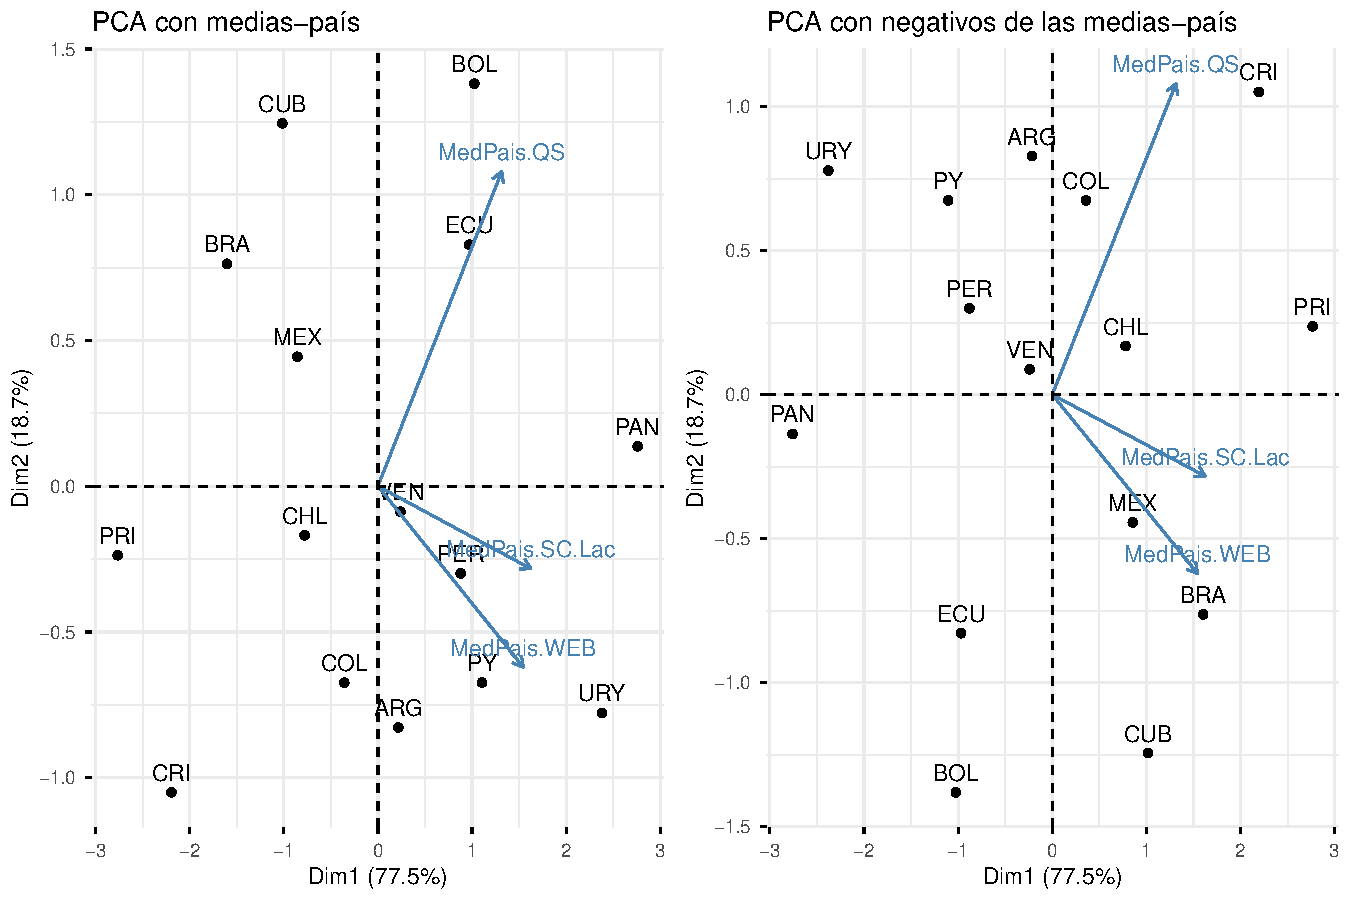
\includegraphics{5_ACP_19_04_2026_diapositivas-008}
	\caption{Representación simultánea de países y rankings promedio por países. IZquierda con promedios originales: PRI, BRA, CUB, MEX y CRI se encuentran en el lado opuesto de las medias-país en el ranking Scimago. Derecha con los negativos de los promedios: estos mismos países se encuentran hacia el mismo lado que apuntan los vectores con las medias-país}\label{fig:rloriginales}
\end{figure}
\end{frame}

\begin{frame}{ACP medias por país: Calidad de la representación}
\begin{table}[!h]
\centering
\caption{\label{tab:vprankis}Valores propios, porcentajes de varianza
      y de varianza acumulados}
\centering
\resizebox{\ifdim\width>\linewidth\linewidth\else\width\fi}{!}{
\begin{tabular}[t]{lrrr}
\toprule
  & eigenvalue & percentage of variance & cumulative percentage of variance\\
\midrule
\cellcolor{gray!10}{comp 1} & \cellcolor{gray!10}{2.325} & \cellcolor{gray!10}{77.517} & \cellcolor{gray!10}{77.517}\\
comp 2 & 0.562 & 18.723 & 96.240\\
\cellcolor{gray!10}{comp 3} & \cellcolor{gray!10}{0.113} & \cellcolor{gray!10}{3.760} & \cellcolor{gray!10}{100.000}\\
\bottomrule
\end{tabular}}
\end{table}\end{frame}

\begin{frame}{ACP medias por país: Plano 1-2 primeros dos factores}
\setkeys{Gin}{width=0.4\textwidth} % para redefinir el tama?o de los graficos
\begin{figure}[H]
	\centering
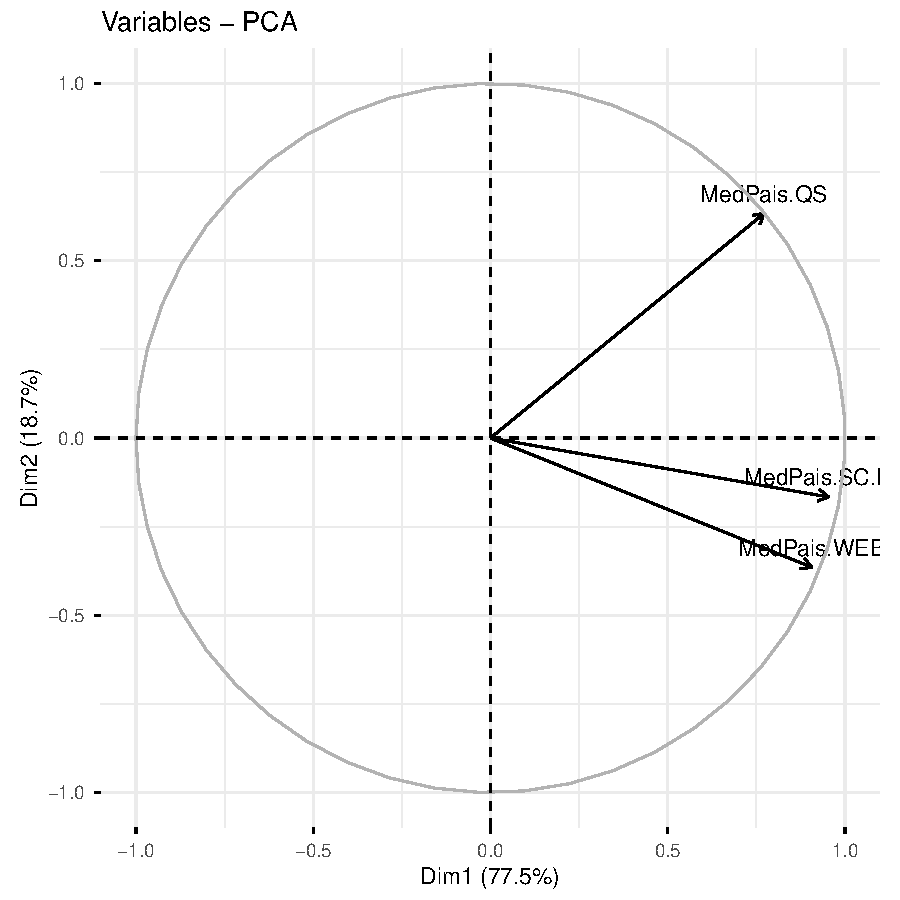
\includegraphics{5_ACP_19_04_2026_diapositivas-010}
	\caption{Proyección de los tres rankings sobre el plano formado por los dos primeros factores. Scimago y WebRanking muestran alta asociación entre ellos, pero asocian muy poco o nada con el Qs}\label{fig:Tresrankvar}
\end{figure}
\end{frame}

\begin{frame}{ACP medias por país: tres indicadores básicos para las interpretaciones}
\begin{table}[!h]
\centering
\caption{\label{tab:CargasFactvar}coordenadas de las variables (Cargas factoriales)}
\centering
\begin{tabular}[t]{lrrr}
\toprule
  & Dim.1 & Dim.2 & Dim.3\\
\midrule
\cellcolor{gray!10}{MedPais.SC.Lac} & \cellcolor{gray!10}{0.954} & \cellcolor{gray!10}{-0.166} & \cellcolor{gray!10}{-0.251}\\
MedPais.QS & 0.772 & 0.633 & 0.058\\
\cellcolor{gray!10}{MedPais.WEB} & \cellcolor{gray!10}{0.906} & \cellcolor{gray!10}{-0.364} & \cellcolor{gray!10}{0.215}\\
\bottomrule
\end{tabular}
\end{table}
\end{frame}

\begin{frame}{..}
\begin{table}[!h]
\centering
\caption{\label{tab:COntribrankis}Contribuciones}
\centering
\begin{tabular}[t]{lrrr}
\toprule
  & Dim.1 & Dim.2 & Dim.3\\
\midrule
\cellcolor{gray!10}{MedPais.SC.Lac} & \cellcolor{gray!10}{39.097} & \cellcolor{gray!10}{4.923} & \cellcolor{gray!10}{55.980}\\
MedPais.QS & 25.605 & 71.429 & 2.967\\
\cellcolor{gray!10}{MedPais.WEB} & \cellcolor{gray!10}{35.298} & \cellcolor{gray!10}{23.648} & \cellcolor{gray!10}{41.054}\\
\bottomrule
\end{tabular}
\end{table}\end{frame}

\begin{frame}{..}
\begin{table}[!h]
\centering
\caption{\label{tab:cosedos}Cosenos cuadrados para las variables}
\centering
\begin{tabular}[t]{lrrr}
\toprule
  & Dim.1 & Dim.2 & Dim.3\\
\midrule
\cellcolor{gray!10}{MedPais.SC.Lac} & \cellcolor{gray!10}{0.909} & \cellcolor{gray!10}{0.028} & \cellcolor{gray!10}{0.063}\\
MedPais.QS & 0.595 & 0.401 & 0.003\\
\cellcolor{gray!10}{MedPais.WEB} & \cellcolor{gray!10}{0.821} & \cellcolor{gray!10}{0.133} & \cellcolor{gray!10}{0.046}\\
\bottomrule
\end{tabular}
\end{table}\end{frame}

\begin{frame}{Interpretación del plano 1-2}
\begin{center}
\begin{figure}[H]
\centering
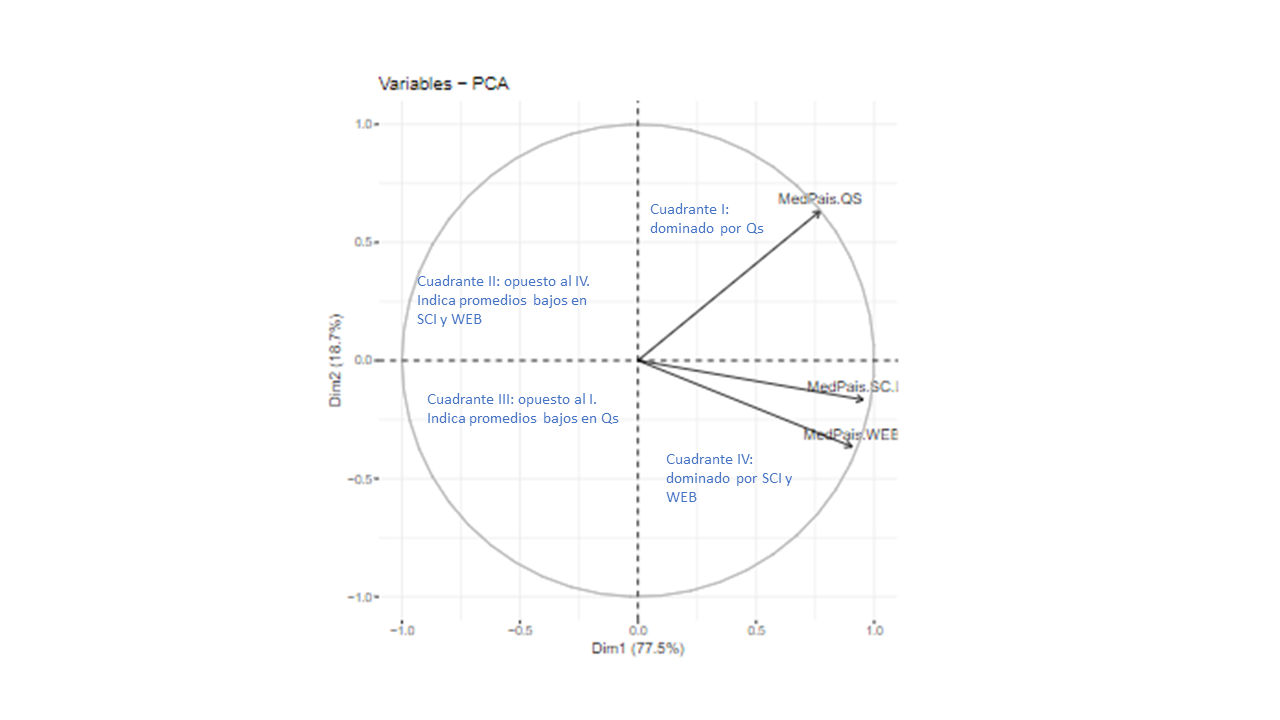
\includegraphics[width=1\textwidth]{PlanoINtrepretado}
% \caption{Causas de muerte en la guerra}
\end{figure}
\label{fig:planointerpretado}
\end{center}

\end{frame}

\begin{frame}{Tipificación de los objetos}
\begin{table}[!h]
\centering
\caption{\label{tab:CargasFact}Coordenadas de los objetos (ciudades)}
\centering
\fontsize{7}{9}\selectfont
\begin{tabular}[t]{lrrr}
\toprule
  & Dim.1 & Dim.2 & Dim.3\\
\midrule
\cellcolor{gray!10}{PRI} & \cellcolor{gray!10}{2.77} & \cellcolor{gray!10}{0.24} & \cellcolor{gray!10}{-0.04}\\
CRI & 2.19 & 1.05 & 0.42\\
\cellcolor{gray!10}{BRA} & \cellcolor{gray!10}{1.60} & \cellcolor{gray!10}{-0.76} & \cellcolor{gray!10}{-0.39}\\
CUB & 1.02 & -1.24 & -0.21\\
\cellcolor{gray!10}{MEX} & \cellcolor{gray!10}{0.86} & \cellcolor{gray!10}{-0.44} & \cellcolor{gray!10}{-0.26}\\
\addlinespace
CHL & 0.78 & 0.17 & -0.22\\
\cellcolor{gray!10}{COL} & \cellcolor{gray!10}{0.36} & \cellcolor{gray!10}{0.67} & \cellcolor{gray!10}{0.22}\\
ARG & -0.22 & 0.83 & -0.13\\
\cellcolor{gray!10}{VEN} & \cellcolor{gray!10}{-0.24} & \cellcolor{gray!10}{0.09} & \cellcolor{gray!10}{-0.17}\\
PER & -0.88 & 0.30 & 0.01\\
\addlinespace
\cellcolor{gray!10}{ECU} & \cellcolor{gray!10}{-0.97} & \cellcolor{gray!10}{-0.83} & \cellcolor{gray!10}{0.75}\\
BOL & -1.02 & -1.38 & 0.31\\
\cellcolor{gray!10}{PY} & \cellcolor{gray!10}{-1.11} & \cellcolor{gray!10}{0.67} & \cellcolor{gray!10}{0.41}\\
URY & -2.38 & 0.78 & -0.45\\
\cellcolor{gray!10}{PAN} & \cellcolor{gray!10}{-2.76} & \cellcolor{gray!10}{-0.14} & \cellcolor{gray!10}{-0.26}\\
\bottomrule
\end{tabular}
\end{table}\end{frame}

\begin{frame}{..}
\begin{table}[!h]
\centering
\caption{\label{tab:ContribrankisInd}Contribuciones de los países (objetos)}
\centering
\fontsize{7}{9}\selectfont
\begin{tabular}[t]{lrrr}
\toprule
  & Dim.1 & Dim.2 & Dim.3\\
\midrule
\cellcolor{gray!10}{PRI} & \cellcolor{gray!10}{21.928} & \cellcolor{gray!10}{0.666} & \cellcolor{gray!10}{0.118}\\
BRA & 7.364 & 6.908 & 8.982\\
\cellcolor{gray!10}{CUB} & \cellcolor{gray!10}{2.961} & \cellcolor{gray!10}{18.386} & \cellcolor{gray!10}{2.579}\\
MEX & 2.099 & 2.338 & 3.846\\
\cellcolor{gray!10}{CRI} & \cellcolor{gray!10}{13.790} & \cellcolor{gray!10}{13.100} & \cellcolor{gray!10}{10.539}\\
\addlinespace
CHL & 1.741 & 0.337 & 2.838\\
\cellcolor{gray!10}{VEN} & \cellcolor{gray!10}{0.165} & \cellcolor{gray!10}{0.091} & \cellcolor{gray!10}{1.803}\\
COL & 0.368 & 5.396 & 2.950\\
\cellcolor{gray!10}{ARG} & \cellcolor{gray!10}{0.134} & \cellcolor{gray!10}{8.139} & \cellcolor{gray!10}{0.996}\\
BOL & 3.008 & 22.633 & 5.842\\
\addlinespace
\cellcolor{gray!10}{PER} & \cellcolor{gray!10}{2.220} & \cellcolor{gray!10}{1.065} & \cellcolor{gray!10}{0.003}\\
ECU & 2.688 & 8.147 & 33.509\\
\cellcolor{gray!10}{PY} & \cellcolor{gray!10}{3.504} & \cellcolor{gray!10}{5.393} & \cellcolor{gray!10}{10.002}\\
URY & 16.218 & 7.180 & 12.056\\
\cellcolor{gray!10}{PAN} & \cellcolor{gray!10}{21.812} & \cellcolor{gray!10}{0.222} & \cellcolor{gray!10}{3.936}\\
\bottomrule
\end{tabular}
\end{table}\end{frame}

\begin{frame}{..}
\begin{table}[!h]
\centering
\caption{\label{tab:cosedosIND}Cosenos cuadrados para los países (objetos)}
\centering
\fontsize{7}{9}\selectfont
\begin{tabular}[t]{lrrr}
\toprule
  & Dim.1 & Dim.2 & Dim.3\\
\midrule
\cellcolor{gray!10}{PRI} & \cellcolor{gray!10}{0.992} & \cellcolor{gray!10}{0.007} & \cellcolor{gray!10}{0.000}\\
BRA & 0.778 & 0.176 & 0.046\\
\cellcolor{gray!10}{CUB} & \cellcolor{gray!10}{0.393} & \cellcolor{gray!10}{0.590} & \cellcolor{gray!10}{0.017}\\
MEX & 0.736 & 0.198 & 0.065\\
\cellcolor{gray!10}{CRI} & \cellcolor{gray!10}{0.790} & \cellcolor{gray!10}{0.181} & \cellcolor{gray!10}{0.029}\\
\addlinespace
CHL & 0.888 & 0.042 & 0.070\\
\cellcolor{gray!10}{VEN} & \cellcolor{gray!10}{0.600} & \cellcolor{gray!10}{0.080} & \cellcolor{gray!10}{0.319}\\
COL & 0.203 & 0.718 & 0.079\\
\cellcolor{gray!10}{ARG} & \cellcolor{gray!10}{0.063} & \cellcolor{gray!10}{0.915} & \cellcolor{gray!10}{0.022}\\
BOL & 0.343 & 0.624 & 0.032\\
\addlinespace
\cellcolor{gray!10}{PER} & \cellcolor{gray!10}{0.896} & \cellcolor{gray!10}{0.104} & \cellcolor{gray!10}{0.000}\\
ECU & 0.428 & 0.313 & 0.259\\
\cellcolor{gray!10}{PY} & \cellcolor{gray!10}{0.662} & \cellcolor{gray!10}{0.246} & \cellcolor{gray!10}{0.092}\\
URY & 0.875 & 0.094 & 0.032\\
\cellcolor{gray!10}{PAN} & \cellcolor{gray!10}{0.989} & \cellcolor{gray!10}{0.002} & \cellcolor{gray!10}{0.009}\\
\bottomrule
\end{tabular}
\end{table}\end{frame}

\begin{frame}{Distancia entre objetos}
\setkeys{Gin}{width=0.4\textwidth} % para redefinir el tama?o de los graficos
\begin{figure}[H]
	\centering
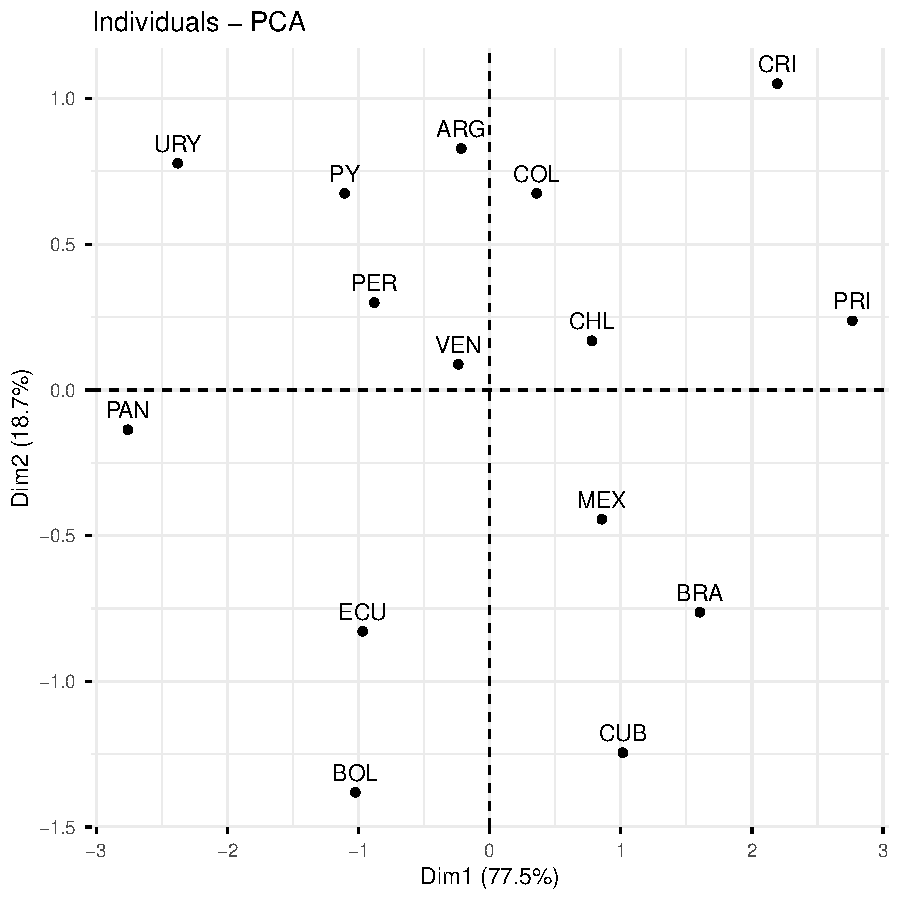
\includegraphics{5_ACP_19_04_2026_diapositivas-017}
	\caption{Proyección de los países sobre los dos primeros factores. Sobresalen en los extremos Cuba, Brasil, Puerto Rico, Costa Rica en el lado derecho del plano y Uruguay, Panamá y Bolivia en el lado derecho.}\label{fig:Tresrankpaises}
\end{figure}
\end{frame}

\begin{frame}{Relaciones entre objetos y variables: biplots}
\setkeys{Gin}{width=0.5\textwidth} % para redefinir el tama?o de los graficos
\begin{figure}[H]
	\centering
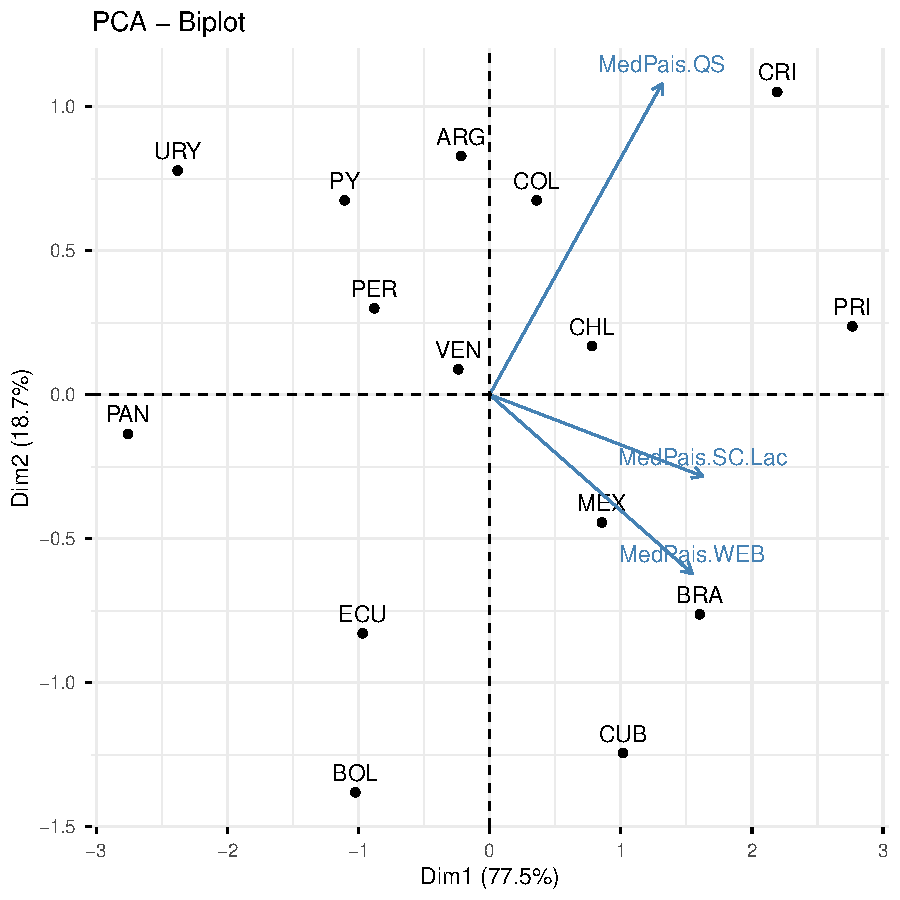
\includegraphics{5_ACP_19_04_2026_diapositivas-018}
	\caption{Representación simultánea de los rankings y los paises}\label{fig:BiploRankpaises}
\end{figure}

\end{frame}

\begin{frame}{Objetos suplementarios o ilustrativos}
Son objetos a los que se observaron las mismas variables que a los objetos activos,
pero que posiblemente pertenecen a otra población objetivo.
\end{frame}

\begin{frame}{Objetos suplementarios o ilustrativos}
También se pueden utilizar como objetos ilustrativos algunos objetos que, siendo parte del grupo observado,
son casos atípicos, como se muestra a continuación con algunos países de características especiales
como Bolivia, Cuba, Puerto Rico y Paraguay, que solo tienen una universidad y que, por esta razón,
podrían haber distorsionado los planos factoriales del análisis.
\end{frame}



\begin{frame}{Objetos ilustrativos}
\setkeys{Gin}{width=0.6\textwidth} % para redefinir el tama?o de los graficos
\begin{figure}[H]
	\centering
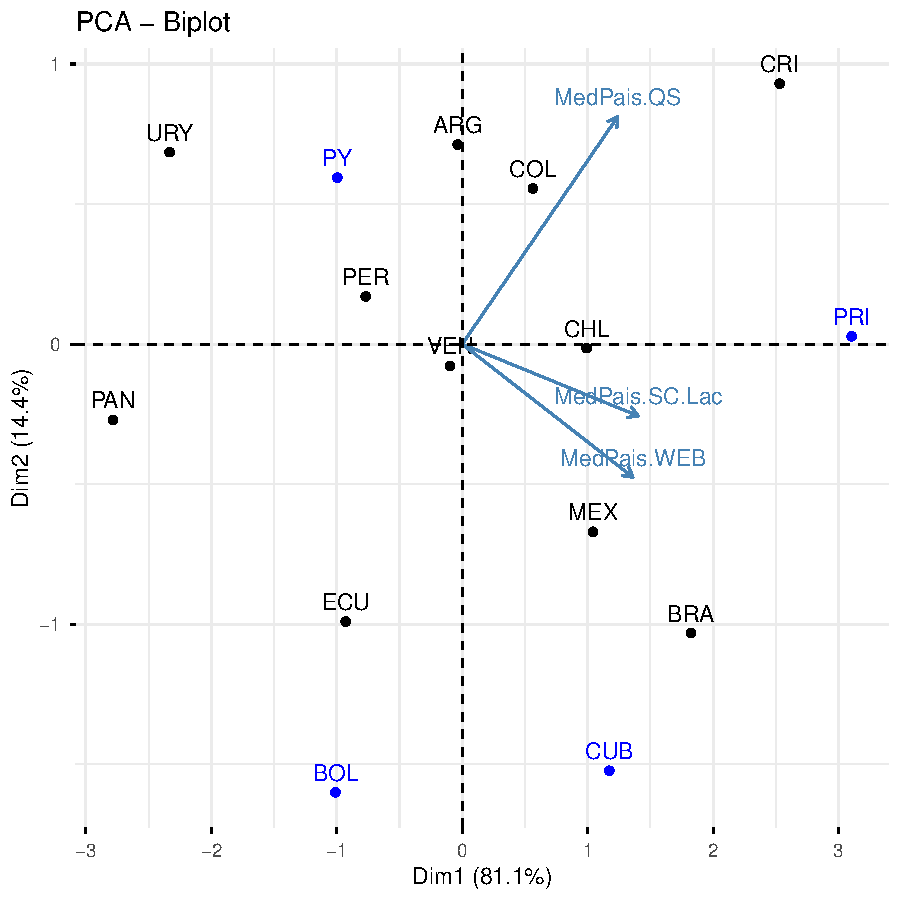
\includegraphics{5_ACP_19_04_2026_diapositivas-020}
	\caption{Paises con una sola univresidad como objetos ilustrativos}\label{fig:BiploRankpaisesILUSTRATIVOS}
\end{figure}
\end{frame}

\begin{frame}{Variables suplementarias o ilustrativas}
Son variables que han sido observadas en los mismos objetos del análisis original, pero posiblemente con otros objetivos. Éstas naturalmente no hacen parte de la construcción de las componentes, pero pueden ilustrar, complementar y enrriquecer el análisis. 

Tambien pueden utililzarse para la validación de índices o indicadores construidos con criterios externos, como en el caso que se presenta en el ejemplo \ref{rankines}.
\end{frame}

\begin{frame}{Ejemplo: Validación de indicadores como variables ilustrativas}
(Variables suplementarias) La mayoría de los rankings de universidades se construyen a partir de unos criterios predefinidos por la entidad que los produce, criterios a los cuales \textbf{se asignan ponderaciones justificadas conceptualmente}, con la intención de que tanto los criterios como los rankings asignados a las universidades sean \textbf{comparables}. 
\end{frame}

\begin{frame}{..}
Para validar dichas ponderaciones suelen utilizarse criterios estadísticos basados por ejemplo en el ACP como se ilustra en este ejemplo.

Se realiza un ACP a los criterios con los que se construye el ARWU y se proyectan como variables suplementarias los rankings nacional, regional y mundial, así como el puntaje total (Total Score) que da origen al ranking de las universidades. 
\end{frame}


\begin{frame}{..}
\begin{table}[!h]
\centering
\caption{\label{tab:validArwu}Correlaciones, contribuciones y cosenos cuadrados}
\centering
\fontsize{7}{9}\selectfont
\begin{tabular}[t]{lrrrrrr}
\toprule
\multicolumn{1}{c}{ } & \multicolumn{2}{c}{Coord} & \multicolumn{2}{c}{Contr} & \multicolumn{2}{c}{Cos2} \\
\cmidrule(l{3pt}r{3pt}){2-3} \cmidrule(l{3pt}r{3pt}){4-5} \cmidrule(l{3pt}r{3pt}){6-7}
  & Factor 1 & Factor 2 & Factor 1 & Factor 2 & Factor 1 & Factor 2\\
\midrule
\cellcolor{gray!10}{Alumni} & \cellcolor{gray!10}{0.81} & \cellcolor{gray!10}{-0.29} & \cellcolor{gray!10}{16.75} & \cellcolor{gray!10}{7.48} & \cellcolor{gray!10}{0.65} & \cellcolor{gray!10}{0.09}\\
Award & 0.84 & -0.40 & 18.18 & 14.03 & 0.70 & 0.16\\
\cellcolor{gray!10}{HiCi} & \cellcolor{gray!10}{0.84} & \cellcolor{gray!10}{0.37} & \cellcolor{gray!10}{18.40} & \cellcolor{gray!10}{11.62} & \cellcolor{gray!10}{0.71} & \cellcolor{gray!10}{0.13}\\
N.S & 0.92 & 0.21 & 21.93 & 3.70 & 0.85 & 0.04\\
\cellcolor{gray!10}{PUB} & \cellcolor{gray!10}{0.58} & \cellcolor{gray!10}{0.73} & \cellcolor{gray!10}{8.62} & \cellcolor{gray!10}{46.37} & \cellcolor{gray!10}{0.33} & \cellcolor{gray!10}{0.54}\\
\addlinespace
PCP & 0.79 & -0.44 & 16.12 & 16.80 & 0.62 & 0.19\\
\bottomrule
\end{tabular}
\end{table}\end{frame}

\begin{frame}{..}
\setkeys{Gin}{width=0.6\textwidth} % para redefinir el tama?o de los graficos
\begin{figure}[H]
	\centering
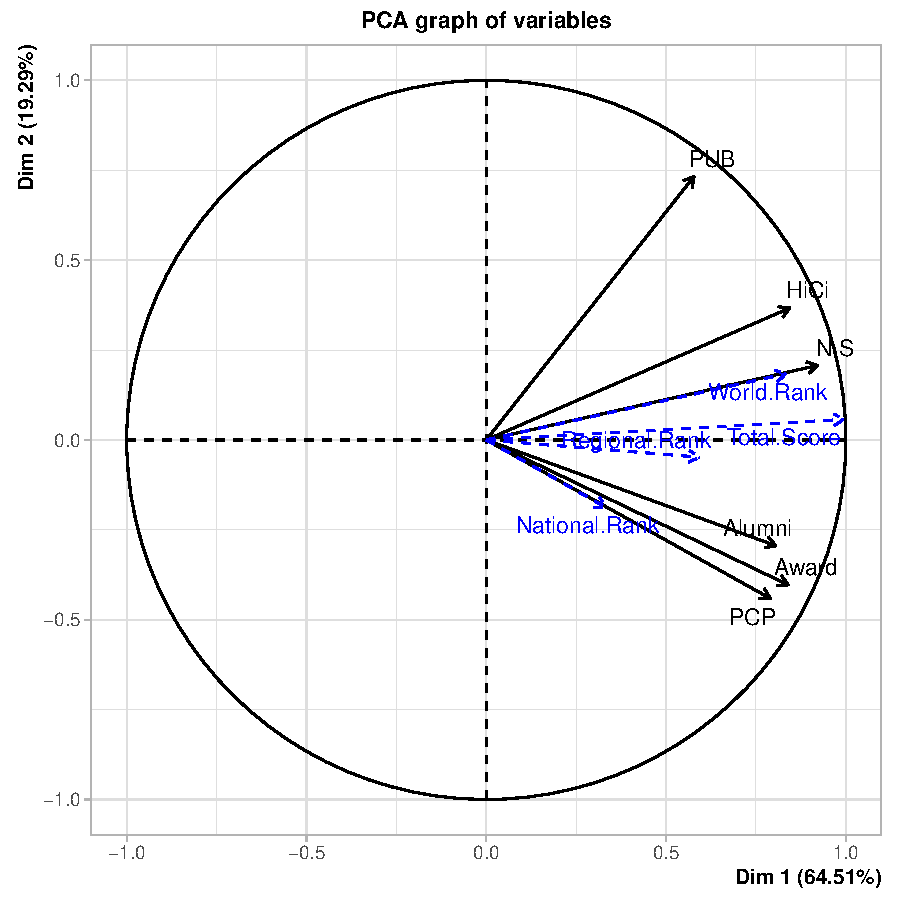
\includegraphics{5_ACP_19_04_2026_diapositivas-023}
		\caption{Indicadores del ARWU sobre el plano 1-2}\label{fig:arwupl_1_2}
\end{figure}
\end{frame}



\begin{frame}{Objetos ilustrativos}
 
\begin{table}[!h]
\centering
\caption{\label{tab:rankinsReord}Negativos de los puestos de las universidades colombianas que quedaron entre los primeros 149 puestos del ranking QS}
\centering
\fontsize{7}{9}\selectfont
\begin{tabular}[t]{lrrrl}
\toprule
  & SC.Reord & Qs.Reord & Web.Reord & Estatus\\
\midrule
\cellcolor{gray!10}{LOS ANDES} & \cellcolor{gray!10}{-3} & \cellcolor{gray!10}{-1} & \cellcolor{gray!10}{-3} & \cellcolor{gray!10}{Pri}\\
NACIONAL & -1 & -2 & -1 & Pub\\
\cellcolor{gray!10}{ANTIOQUIA} & \cellcolor{gray!10}{-2} & \cellcolor{gray!10}{-3} & \cellcolor{gray!10}{-2} & \cellcolor{gray!10}{Pub}\\
JAVERIANA & -5 & -4 & -4 & Pri\\
\cellcolor{gray!10}{ROSARIO} & \cellcolor{gray!10}{-7} & \cellcolor{gray!10}{-5} & \cellcolor{gray!10}{-7} & \cellcolor{gray!10}{Pri}\\
\addlinespace
DEL VALLE & -4 & -6 & -5 & Pub\\
\cellcolor{gray!10}{LA SABANA} & \cellcolor{gray!10}{-10} & \cellcolor{gray!10}{-7} & \cellcolor{gray!10}{-10} & \cellcolor{gray!10}{Pri}\\
UIS & -6 & -8 & -6 & Pub\\
\cellcolor{gray!10}{DEL NORTE} & \cellcolor{gray!10}{-14} & \cellcolor{gray!10}{-9} & \cellcolor{gray!10}{-11} & \cellcolor{gray!10}{Pri}\\
EAFIT & -9 & -10 & -8 & Pri\\
\addlinespace
\cellcolor{gray!10}{PT BOLIVARIA} & \cellcolor{gray!10}{-8} & \cellcolor{gray!10}{-11} & \cellcolor{gray!10}{-9} & \cellcolor{gray!10}{Pri}\\
EXTERNADO & -13 & -12 & -14 & Pri\\
\cellcolor{gray!10}{TADEO} & \cellcolor{gray!10}{-11} & \cellcolor{gray!10}{-13} & \cellcolor{gray!10}{-12} & \cellcolor{gray!10}{Pri}\\
LA SALLE & -12 & -14 & -13 & Pri\\
\bottomrule
\end{tabular}
\end{table}\end{frame}


\begin{frame}{Objetos ilustrativos}
\setkeys{Gin}{width=1.6\textwidth, height=0.8\textheight,keepaspectratio} % para redefinir el tamaño de los graficos
\begin{figure}[H]
	\centering
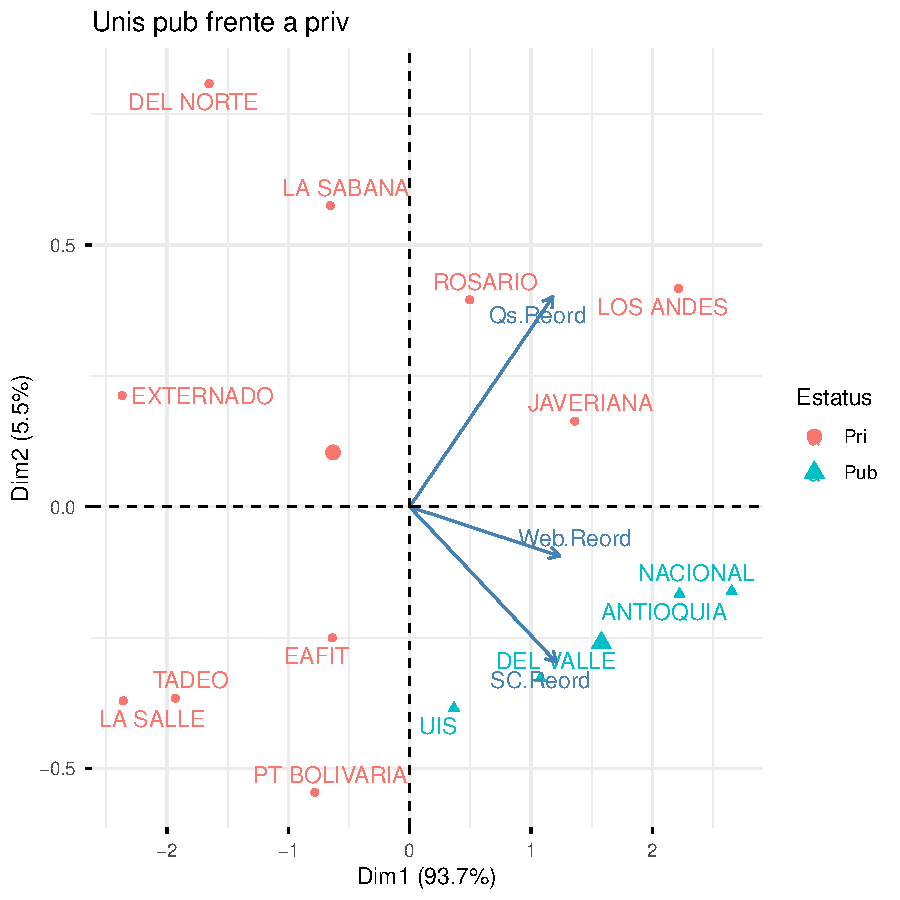
\includegraphics{5_ACP_19_04_2026_diapositivas-027}
	\caption{Universidades privadas proyectadas como ilustrativas sobre el plamo 1-2, construido con las universidades públicas}\label{fig:rankUnis}
\end{figure}
\end{frame}

\begin{frame}{Construcción y obtención de las componentes. Método de multiplicadores de Lagrange:}
Para una matriz simétrica $B$, consiste en buscar inicialmente un valor $\lambda_1$ y un vector $u_1$ que maximice una forma cuadrática $u_1^{\prime} B u_1$ sujeto a la restricción $\lambda_1 u_1^{\prime} u_1$:
\begin{equation}\label{lagrange1}
\mathcal{L}=u_1^{\prime} B u_1-\lambda_1 u_1^{\prime} u_1 = u_1^{\prime}(Bu_1-\lambda_1 u_1)=0
\end{equation}
la cual permite encontrar un vector $u_1\ne 0$ normado $u_1^\prime u_1=1$. Si $u_1\ne0$ entonces  (\ref{lagrange1}) se cumple cuando $Bu_1-\lambda_1 u_1 = 0$ y por tanto cuando:
\begin{equation}\label{lagrange2}
Bu_1 = \lambda_1 u_1
\end{equation}
expresión que coincide con la definición de $\lambda_1$ y $u_1$ como valor y vector propio de $B$ respectivamente.
\end{frame}


\begin{frame}{Método de multiplicadores de Lagrange:}
Procediendo iterativamente se puede encontrar el 

segundo vector $u_2$ ortogonal a $u_1$ ($u_2^\prime u_1=0$) que maximiza $u_2^{\prime} Bu_2$ 

sujeto a las restricciones $u_2^\prime u_1=0$ y $u_2^\prime u_2=1$,

cuya solución $u_2$ es aquel vector propio $B$ que corresponde a su segundo mayor valor propio de $B$ que satisface  
$$\lambda_1 \ge \lambda_2.$$
y por tanto 
\[Bu_2 = u_2\lambda_2\]
Este proceso se puede continuar hasta encontrar $u_1,\ldots,u_p$ vectores propios de $B$ unitarios y ortogonales con sus correspondientes valores propios no nulos con la propiedad:
$$\lambda_1 \ge \lambda_2 \ge \cdots \ge \lambda_p$$.
\end{frame}

\begin{frame}{Cálculo de los valores y vectores propios de la matriz de correlación}
Reemplazando $B$ en (\ref{lagrange2}) por la matriz de correlación $\mathcal{R}$ se obtiene en general para el $\alpha$-ésimo vector y valor propio (eigenvalue):
$$
Ru_\alpha = \lambda_\alpha u_\alpha , \quad \alpha = 1,\ldots,p
$$
\end{frame}

\begin{frame}{Cálculo de las componentes}
Se define la $\alpha$-ésima componente principal como la proyección de la matriz de datos estandarizados $\widetilde{X}$ sobre el $\alpha$-ésimo vector propio
\begin{equation}\label{TrCoPr1}
\dot{Z}_\alpha = \widetilde{X}^\prime u_\alpha
\end{equation}
La cual tiene varianza 
\begin{equation*}
	V(\dot{Z}_\alpha) = \lambda_\alpha
\end{equation*}
y se puede demostrar que la 
\begin{equation*}
	\textbf{Varianza total} = \sum_{j=1}^{p} s_j^2 = \sum_{\alpha=1}^{p} \lambda_\alpha
\end{equation*}
\end{frame}
% 
% \begin{frame}{..}
% 
% \end{frame}

% 
% \begin{frame}{..}
% 
% \end{frame}

\begin{frame}{LABORATORIO}
El archivo ciudades\_completo\_ago\_2023 tiene las siguientes variables:
\begin{table}[!h]
\centering
\caption{\label{tab:varsCiu}Variables del archivo ciudades completo}
\centering
\fontsize{6}{8}\selectfont
\begin{tabular}[t]{ll}
\toprule
nom1 & nom2\\
\midrule
\cellcolor{gray!10}{CIUDADES} & \cellcolor{gray!10}{Basura.desechos.Ton}\\
Region & PIB.per.capita\\
\cellcolor{gray!10}{Poblacion} & \cellcolor{gray!10}{NBI}\\
Analfabetismo & LinTelx10milH\\
\cellcolor{gray!10}{Cobertura.pria.y.secdaria} & \cellcolor{gray!10}{EElecx10milH}\\
\addlinespace
Cobertura.ed.sup & Acuex10milH\\
\cellcolor{gray!10}{Rel.al.prof} & \cellcolor{gray!10}{Alcantx10milH}\\
N.Gr.Inv..Colcienciasx10milH & GasNatx10milH\\
\cellcolor{gray!10}{No.CeNTROS.Invx10milH} & \cellcolor{gray!10}{Camasx10milH}\\
No.Prf..Doctoradox10milH & HospClinx10milH\\
\addlinespace
\cellcolor{gray!10}{Delitos.M.aMB.y.REC.nat} & \cellcolor{gray!10}{ClientesInternx10milH}\\
Consum.agua.M3 & ProveedInternx10milH\\
\bottomrule
\end{tabular}
\end{table}\end{frame}




\begin{frame}{LAB}
La función PCA dell paquete FactoMineR produce entre otros los siguientes resultados:

\end{frame}

% 
\begin{frame}{LAB continuación}
Utilizar la funcion PCA para contestar las siguientes preguntas:
\begin{enumerate}

  \item Realizar un ACP para la tabla de ciudades con las siguientes variables: LinTelx10milH, , EElecx10milH, , Acuex10milH, , Alcantx10milH, GasNatx10milH, Camasx10milH, HospClinx10milH, ClientesInternx10milH, ProveedInternx10milH \label{ACP1}.

   \item Incluir la variable \textbf{Poblacion} en el análisis y repetir los ejercicios (\ref{primero})  a (\ref{ultimo}) indicando en cada caso si hubo cambios con la inclusión de la nueva variable.
   
   \item Incluir como ilustrativas las variables Poblacion, Analfabetismo, Cobertura.pria.y.secdaria, Cobertura.ed.sup, Rel.al.prof, y repetir los ejercicios (\ref{primero})  a (\ref{ultimo}) (Sugerencia: para incluir las ilustrativas usar el comando \textbf{quanti.sup =} de la función PCA)
\end{enumerate}   

\end{frame}


% 
% \begin{frame}
% \frametitle{Referencias}
% \bibliography{BiblioMultivariado}
% \end{frame}
% 
% \begin{frame}{..}
% 
% \end{frame}
% 
% \begin{frame}{..}
% 
% \end{frame}
% 
% \begin{frame}{..}
% 
% \end{frame}


% \begin{frame}[fragile] % esto tocó así porque reporta problema con el FancyVerb se instalaros dos paquetes arriba
% \frametitle{Rankies}
% 
% \end{frame}



\end{document}


